%%%%%%%%%%%%%%%%%%%%%%%%%%%%%%%%%%%%%%%%%
% baposter Landscape Poster
% LaTeX Template
% Version 1.0 (11/06/13)
%
% baposter Class Created by:
% Brian Amberg (baposter@brian-amberg.de)
%
% License:
% CC BY-NC-SA 3.0 (http://creativecommons.org/licenses/by-nc-sa/3.0/)
%
%%%%%%%%%%%%%%%%%%%%%%%%%%%%%%%%%%%%%%%%%

%----------------------------------------------------------------------------------------
% PACKAGES AND OTHER DOCUMENT CONFIGURATIONS
%----------------------------------------------------------------------------------------

\documentclass[landscape,a0paper,fontscale=0.285]{baposter} % Adjust font scale/size

\usepackage{graphicx} % Required for including images
\graphicspath{{figs/}} % Directory in which figures are stored

\usepackage{amsmath} % For typesetting math
\usepackage{amssymb} % Adds new symbols to be used in math mode
\usepackage{mathtools}

\usepackage[numbers]{natbib}

\usepackage{booktabs} % Top and bottom rules for tables
\usepackage{enumitem} % Used to reduce itemize/enumerate spacing
\usepackage{palatino} % Use the Palatino font
\usepackage[font=small,labelfont=bf]{caption} % Required for specifying captions to tables and figures

\usepackage{multicol} % Required for multiple columns
\setlength{\columnsep}{1.5em} % Slightly increase the space between columns
\setlength{\columnseprule}{0mm} % No horizontal rule between columns

\newcommand{\compresslist}{ % Define a command to reduce spacing within itemize enumerate environments, this is used right after \begin{itemize} or \begin{enumerate}
\setlength{\itemsep}{1pt}
\setlength{\parskip}{0pt}
\setlength{\parsep}{0pt}
}

\usepackage[nodisplayskipstretch]{setspace}
\setstretch{0.95}

\newcommand{\D}{\mathcal{D}}
\newcommand{\E}{\mathbb{E}}
\newcommand{\F}{\mathcal{F}}
\newcommand{\M}{\mathcal{M}}
\newcommand{\R}{\mathbb{R}}
\newcommand{\X}{\mathcal{X}}
\newcommand{\like}{\mathcal{L}}
\newcommand{\prob}{\mathbb{P}}
\newcommand{\1}{\mathbbm{1}}

\definecolor{lightblue}{rgb}{0.145,0.6666,1} % Defines color of content box headers

\begin{document}

\begin{poster}
{
headerborder=closed, % Adds a border around the header of content boxes
colspacing=1em, % Column spacing
bgColorOne=white, % Background color for the gradient on the left side of the poster
bgColorTwo=white, % Background color for the gradient on the right side of the poster
borderColor=lightblue, % Border color
headerColorOne=black, % Background color for the header in the content boxes (left side)
headerColorTwo=lightblue, % Background color for the header in the content boxes (right side)
headerFontColor=white, % Text color for the header text in the content boxes
boxColorOne=white, % Background color of the content boxes
textborder=roundedleft, % Format of the border around content boxes, can be: none, bars, coils, triangles, rectangle, rounded, roundedsmall, roundedright or faded
eyecatcher=true, % Set to false for ignoring the left logo in the title and move the title left
headerheight=0.1\textheight, % Height of the header
headershape=roundedright, % Specify the rounded corner in the content box headers, can be: rectangle, small-rounded, roundedright, roundedleft or rounded
headerfont=\Large\bf\textsc, % Large, bold and sans serif font in the headers of content boxes
%textfont={\setlength{\parindent}{1.5em}}, % Uncomment for paragraph indentation
linewidth=2pt % Width of the border lines around content boxes
}
%-------------------------------------------------------------------------------
% TITLE SECTION
%-------------------------------------------------------------------------------
%
{
\includegraphics[height=6.5em]{logo_cal.jpg}} % university/lab logo on left
{\textbf{\LARGE Variance Moderation of Locally Efficient Estimators and
    Supervised Clustering with Applications in High-Dimensional
    Biology\vspace{0.5em}}} % title
{\textsc{Nima S.~Hejazi, Mark J.~van der Laan, \& Alan E.~Hubbard} \hspace{12pt}
  \textit{Graduate Group in Biostatistics}} % Author names and institution
{
\includegraphics[height=9em]{logo_sph.jpg}} % university/lab logo on right

%-------------------------------------------------------------------------------
% OVERVIEW
%-------------------------------------------------------------------------------

\headerbox{Overview \& Motivations}{name=overview,column=0,row=0}{

\begin{itemize}
  \itemsep0.5pt
  \item A general approach for applying variance moderation to locally efficient
    estimators in nonparametric models is introduced.
  \item Variance moderation stabilizes small-sample properties of
    semiparametric-efficient estimators,
    \begin{itemize}
      \itemsep0pt
      \item curbing the error rate of tests relative to classical approaches
      \item and facilitating \textit{supervised clustering} from derived
        association profiles.
    \end{itemize}
  \item Focusing on a targeted maximum likelihood estimator (TMLE), we
    illustrate how the proposed approach generalizes readily to any
    asymptotically linear estimator.
  \item The \underline{\texttt{biotmle} R package} \cite{hejazi2017biotmle}
    implements the inference and clustering methods, and leverages
    state-of-the-art machine learning.
\end{itemize}

}

%-------------------------------------------------------------------------------
% INTRODUCTION
%-------------------------------------------------------------------------------

\headerbox{Data: Benzene Biomarkers}
{name=introduction,column=1,row=0,bottomaligned=overview}{

\begin{itemize}
  \itemsep1pt
  \item There is a pressing need for model-free, technology-agnostic statistical
    methods for analyzing multiple kinds of exposome data.
  \item We consider a data from an occupational exposure study, generated by the
    \textit{Illumina Human Ref-8 BeadChips} platform.
  \item Baseline (phenotypic) confounders and exposure status were collected for
    $n = 125$ participants, alongside expression measures for $\sim 22,000$
    genes.
  \item Baseline covariates ($W$): age, sex, and smoking status.
  \item Exposure ($A$): degree of Benzene exposure (none, $<1$ppm, $>5$ppm).
  \item Outcome ($Y = (Y_b: b = 1, \ldots, B)$): vector of gene expression
    measures, after full qunatile normalization.
\end{itemize}

}

%-------------------------------------------------------------------------------
% METHODS 2: Supervised Clustering
%-------------------------------------------------------------------------------
\headerbox{Methodology II: Supervised Distance Matrices}{name=results,column=2,span=2,row=0}{

\begin{itemize}
  \itemsep0.75pt
  \item Let $\phi: (W, A, Y) \mapsto D_b(P_0)(O)$ be the EIF transformation,
    where $D_b(P_0)(O_i)$ is the contribution of subject $i$ to the estimate of
    the biomarker-specific target parameter $\Psi_{b,n}$.
  \item $Z = \phi(W, A, Y)$ is then a $B \times N$ matrix, where each entry
    $(b,i)$ may be interpreted as the degree to which subject $i$ deviates from
    the target parameter $\Psi_{b,n}$ \cite{hejazi2018+supervised}, and is thus
    an \textit{association profile}.
  \item A \textit{supervised distance matrix} \cite{pollard2008supervised}
    may be constructed by applying an appropriate distance metric of choice
    (e.g., Euclidean, correlation) to the transformed values $Z$.
  \item $\widetilde{T}(Z)$, the resultant $B \times B$ empirical distance
    matrix, encodes the dissimilarity between pairs of biomarker association
    profiles.
  \item When $\widetilde{T}(b,b')$ is small, the biomarkers $b$ and $b'$ have
    similar contriubtions to the target parameter $\Psi$, across the $n$
    subjects.
  \item \textit{Supervised clustering} may be performed by applying standard
    clustering algorithms to the matrix $\widetilde{T}$, thereby finding groups
    of biomarkers that share an association profile w.r.t.~$\Psi$.
  \item In the case of the average treatment effect, a supervised cluster in
    $\widetilde{T}$ of biomarkers is a group whose causal differential
    expression profiles varies similarly with the treatment $A \in \{0, 1\}$.
\end{itemize}
}

%-------------------------------------------------------------------------------
% REFERENCES
%-------------------------------------------------------------------------------

\headerbox{\small References}{name=references,column=2,above=bottom}{
\renewcommand{\section}[2]{\vskip 0.05em} % remove "References" section title
\tiny{ % Reduce the font size in this block
  \setlength{\bibsep}{0.25pt}
  \bibliographystyle{IEEEtran}
  \bibliography{2018_ccb}
  \compresslist
  \vspace{-0.7em}
}
}

%-------------------------------------------------------------------------------
% Contact Information
%-------------------------------------------------------------------------------

\headerbox{\small Contact Information}{name=ack,column=3,aligned=references,above=bottom}{
% This block is as tall as the references block
\begin{itemize}
\itemsep0.25pt
  \item \textbf{N.S.~Hejazi}, Ph.D.~candidate, Group in Biostatistics,
    \textsc{nhejazi@berkeley.edu}
  \item \textbf{M.J.~van der Laan}, Professor of Biostatistics \& Statistics,
    \textsc{laan@berkeley.edu}
  \item \textbf{A.E.~Hubbard}: Professor of Biostatistics,
    \textsc{hubbard@berkeley.edu}
\end{itemize}
}

%-------------------------------------------------------------------------------
% CONCLUSION
%-------------------------------------------------------------------------------

\headerbox{Results}
{name=conclusion,column=2,span=2,row=0,below=results,above=references}{

\vspace{0.25em}

\begin{multicols}{2}

\begin{center}
\vspace*{-0.5cm}
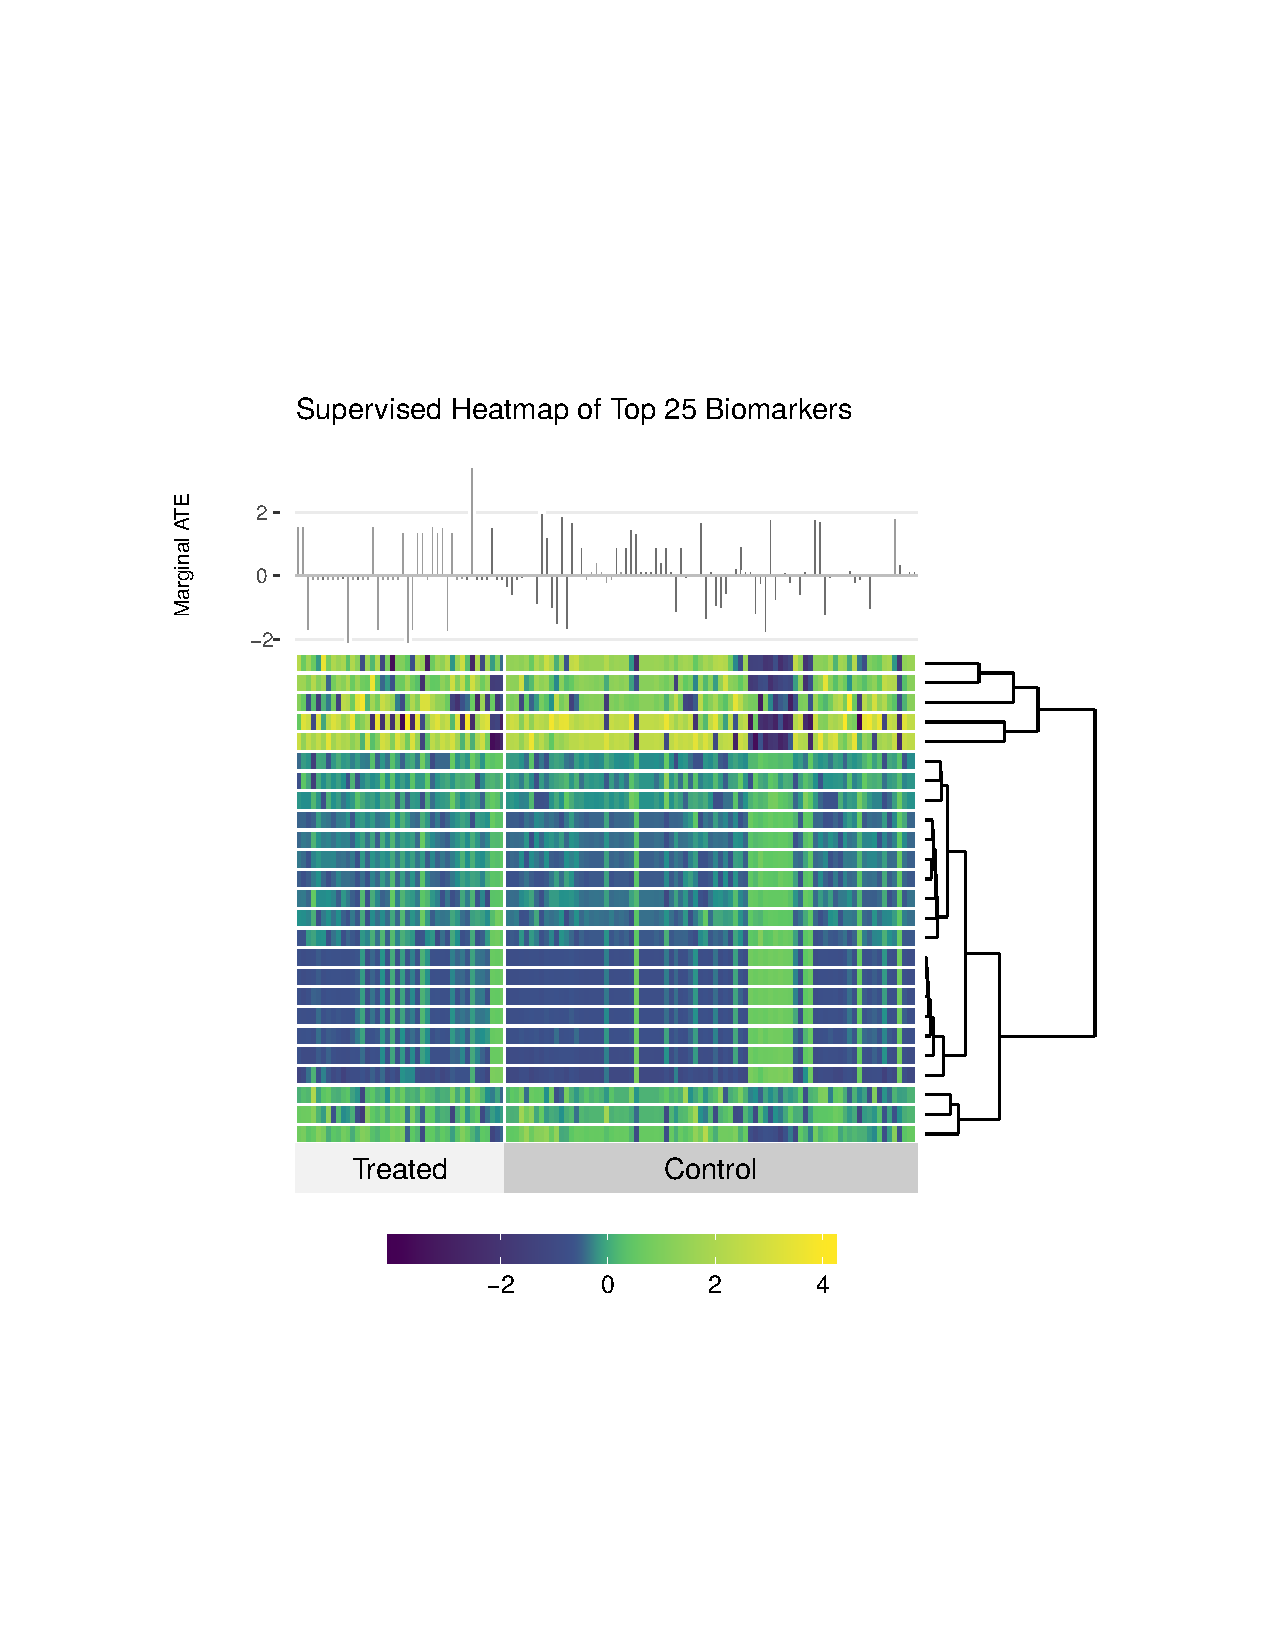
\includegraphics[scale=0.35]{supervised_heatmap}
\captionof{figure}{A \textit{supervised heatmap} of biomarker association
  profiles with the ATE.}
\end{center}

\begin{center}
%\vspace*{-0.49cm}  % CHANGE THIS TO ALIGN IMAGES
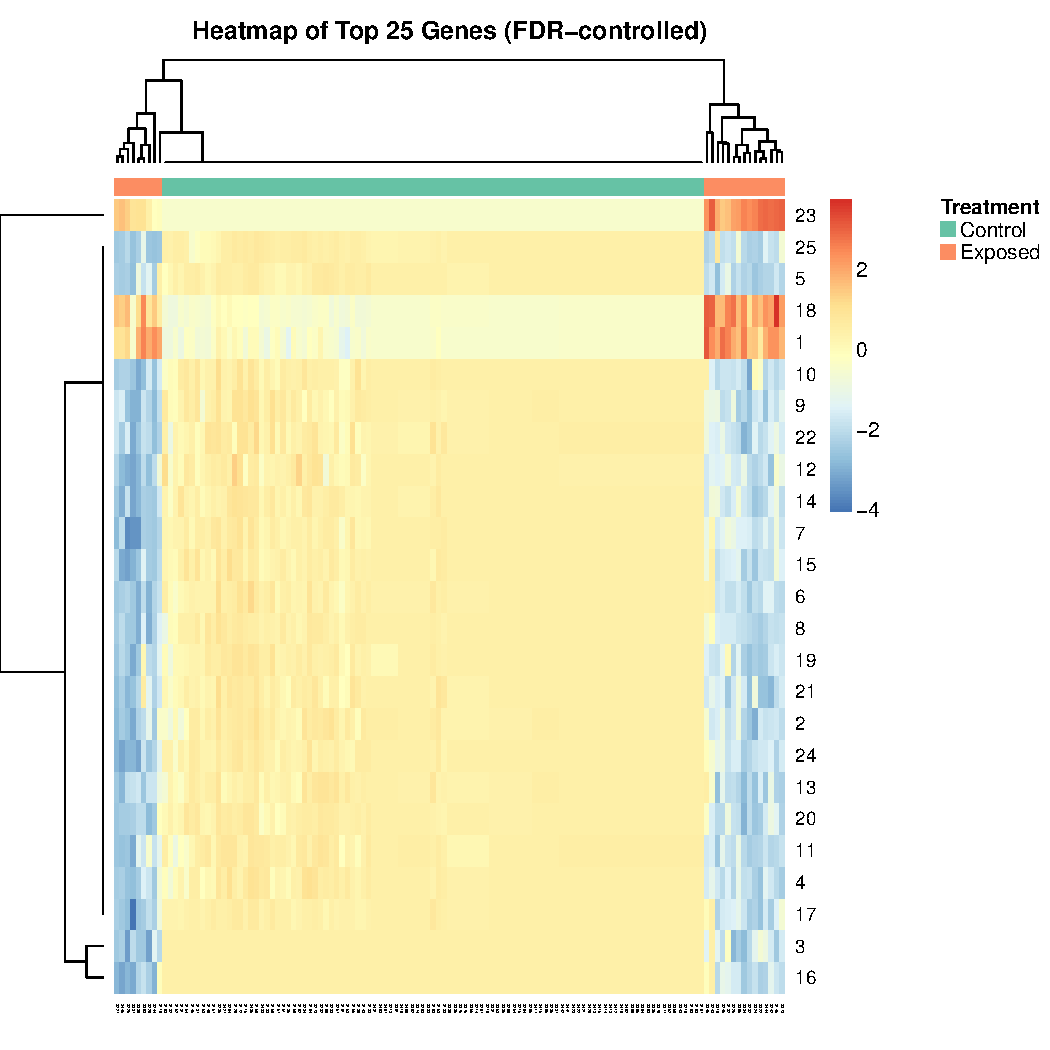
\includegraphics[scale=0.35]{topGenesHeatmap}
\captionof{figure}{Improved error rate control of the variance moderated TMLE
  for the ATE.}
\end{center}

\end{multicols}
}


%-------------------------------------------------------------------------------
% METHODS
%-------------------------------------------------------------------------------

\headerbox{Methodology I: Variance Moderation \& Local Efficiency}{name=method,column=0,span=2,below=overview,bottomaligned=references}{
% This block's bottom aligns with the bottom of the conclusion block

\begin{itemize}
  %\compresslist
  \itemsep0.50pt
  \item Let observed data $O = (W, A, Y) \sim P_0 \in \M$, where $W$ represents
      potential baseline confounders, $A$ the exposure of interest, and
      $Y = ({Y_b}, b = 1, \dots, B)$ a vector of potential biomarkers.
  \item We consider, as an example, the \textit{average treatment effect} (ATE),
      as the causal parameter of interest, which is identified by the observed
      data parameter:
      \begin{equation}\label{ate}
        \Psi_b(P_0) = \E_W[ Q_0^b(A = 1, W) - Q_0^b(A = 0, W)],
      \end{equation}
        where $Q_0^b(A, W) \equiv \E_{P_0}(Y_b \mid A, W)$ and may be estimated
        via \textit{ensemble machine learning}
        \cite{vdl2007super,breiman1996stacked,wolpert1992stacked}.
  %\item To estimate $\Psi$ using the construction from Eqn.~\ref{ate}, a plug-in
    %estimator may be constructed
    %\begin{equation}
      %\Psi_b(P_n) = \frac{1}{n} \sum_{i = 1}^n Q_n^b(A_i = 1, W_i) -
      %Q_n^b(A_i = 0, W_i),
    %\end{equation}
      %where ${Q_n}^b$ is an initial estimate of ${Q_0}^b$ constructed via
      %\textit{ensemble machine learning} \cite{vdl2007super,breiman1996stacked,
      %wolpert1992stacked}.
  \item Like the estimator $\hat{\beta}$ in a linear model $m(A,W \mid \beta)$,
      $\Psi_b(P_n)$ is \textbf{asymptotically linear} (for $\Psi_b$)
      \cite{vdl2011targeted}:
      \begin{equation}\label{asymp_lin}
        \sqrt{n} (\Psi_b(P_n) - \Psi_b(P_0)) = \frac{1}{\sqrt{n}} \sum_{i=1}^n
        D_b(O_i) + o_p(1).
      \end{equation}
  \item $\Psi_b$ has efficient influence function (EIF), relative to the
      nonparametric model $\M$:
      \begin{equation}\label{eif_ate}
        D_b(P_0)(o) = \left(\frac{I(a = 1)}{g(1 \mid w)} -
        \frac{I(a = 0)}{g(0 \mid w)}\right) \cdot \left[y_b - Q_0^b(a, w)\right]
        + \left(Q_0^b(1, w) - Q_0^b(0, w) - \Psi_b(P_0)(o)\right).
      \end{equation}
  \item A moderated test statistic \cite{smyth2004linear,smyth2005limma,
      hejazi2018+supervised} may be constructed for use wiht asymptotically
      linear estimators:
      \begin{equation}\label{mod_eif}
        \widetilde{t}_b = \frac{\sqrt{n}(\Psi_b(P_n) -
          \psi_{\text{null}})}{\widetilde{S}_{b,n}^2}
        \quad \text{where} \quad
        \widetilde{S}_{b,n}^2 = \frac{d_0S_0^2 + d_bS_b^2(D_{b,n})}{d_0 + d_b},
      \end{equation}
    $\{S_b^2, d_b\}$: var.~EIF and df for $b^{th}$ biomarker;
    $\{S_0^2, d_0\}$: var.~EIF and df for other $(B-1)$ biomarkers.
\end{itemize}

}

%-------------------------------------------------------------------------------

\end{poster}

\end{document}
